\documentclass[11pt]{article}
\usepackage[utf8]{inputenc}
\usepackage{algpseudocode}
\usepackage{algorithm}
\usepackage{geometry}
\usepackage{amsfonts}
\usepackage{hyperref}
\usepackage{enumitem}
\usepackage{graphicx}
\usepackage{tabularx}
\usepackage{amsmath}
\usepackage{xcolor}
\usepackage{array}
\usepackage{tikz}
\usetikzlibrary{shapes, arrows}


\title{
    \textbf{CSE564: Reinforcement Learning} \\ \vspace*{-5pt}
    \textbf{\large{Assignment-3}}
}

\author{\href{mailto:divyajeet21529@iiitd.ac.in}{Divyajeet Singh (2021529)}}
\date{\today}

\geometry{a4paper, left=20mm, right=20mm, top=20mm, bottom=20mm}


\begin{document}
    \maketitle

    \section*{Question-1}
    Rewrite the psuedocode of Monte Carlo ES as mentioned in Exercise 5.4. You must explain
    your code and why it is equivalent to the code provided in the book.

    \subsection*{Solution}
    The modified pseudocode of Monte Carlo ES is given in Algorithm \ref{alg:monte-carlo-es}.
    It includes a counter variable $N(s, a)$ for each state-action pair $(s, a)$. Due to the incremental
    nature of the update rule for $Q(s, a)$, the $Returns(s, a)$ function is no longer required.
    The modification can be seen on line \ref{line:update}.
    \begin{algorithm}
        \caption{Monte Carlo ES (Exploring Starts), for estimating $\pi \approx \pi_{*}$}
        \label{alg:monte-carlo-es}
        \begin{algorithmic}[1]
            \Procedure{Monte-carlo-es}{}:
                \State Initialize:
                \Statex \hspace*{26pt} $\pi(s) \in \mathcal{A}(s)$ (arbitrarily), for all $s \in \mathcal{S}$
                \Statex \hspace*{26pt} $Q(s, a) \in \mathbb{R}$ (arbitrarily), for all $s \in \mathcal{S}$, $a \in \mathcal{A}(s)$
                \Statex \hspace*{26pt} $N(s, a) \leftarrow$ 0, for all $s \in \mathcal{S}$, $a \in \mathcal{A}(s)$
                \State Loop forever (for each episode):
                \State \hspace*{26pt} Choose $S_{0} \in \mathcal{S}$ and $A_{0} \in \mathcal{A}(S_{0})$ randomly such that
                all pairs have probability $> 0$
                \State \hspace*{26pt} Generate an episode starting from $S_{0}, A_{0}$, following $\pi$: $S_{0}, A_{0}, R_{1}, \dots, S_{T-1}, A_{T-1}, R_{T}$
                \State \hspace*{26pt} $G \leftarrow 0$
                \State \hspace*{26pt} Loop for each step of episode, $t = T-1, T-2, \dots, 0$:
                \State \hspace*{39pt} $G \leftarrow \gamma G + R_{t+1}$
                \State \hspace*{39pt} Unless the pair $S_{t}, A_{t}$ appears in $S_{0}, A_{0}, S_{1}, A_{1}, \dots, S_{t-1}, A_{t-1}$:
                \State \hspace*{52pt} $N(S_{t}, A_{t}) \leftarrow N(S_{t}, A_{t}) + 1$
                \State \hspace*{52pt} $Q(S_{t}, A_{t}) \leftarrow Q(S_{t}, A_{t}) + \frac{1}{N(S_{t}, A_{t})} \left(G - Q(S_{t}, A_{t}) \right)$ \label{line:update}
                \State \hspace*{52pt} $\pi(S_{t}) \leftarrow \arg\max_{a}Q(S_{t}, a)$
            \EndProcedure
        \end{algorithmic}
    \end{algorithm}
    \vspace*{0pt} \\
    This is equivalent to the psuedocode provided in the book as the update rule for $Q(s, a)$ is the same.
    \begin{align*}
        Q^{(n)}(S_{t}, A_{t}) &= \frac{1}{n} \sum_{i=1}^{n} G^{(i)}(S_{t}, A_{t}) \\
        &= \frac{1}{n} \left( G^{(n)}(S_{t}, A_{t}) + \sum_{i=1}^{n-1} G^{(i)}(S_{t}, A_{t}) \right) \\
        &= \frac{1}{n} \left( G^{(n)}(S_{t}, A_{t}) + (n-1) Q^{(n-1)}(S_{t}, A_{t}) \right) \\
        &= Q^{(n-1)}(S_{t}, A_{t}) + \frac{1}{n} \left( G^{(n)}(S_{t}, A_{t}) - Q^{(n-1)}(S_{t}, A_{t}) \right)
    \end{align*}
    where $G^{(i)}(S_{t}, A_{t})$ and $Q^{(i)}(S_{t}, A_{t})$ are the returns and estimates of $Q(S_{t}, A_{t})$ after $i^{th}$ occurrence of $(S_{t}, A_{t})$.

    \section*{Question-2}
    Draw the backup diagram asked for in exercise 5.3.

    \subsection*{Solution}
    Exercise 5.3 asks for the backup diagram for the Monte Carlo estimation of $q_{\pi}$. The backup diagram is shown in Figure \ref{fig:backup-diagram}.
    This backup diagram is the same as that of the MC estimation of $v_{\pi}$, except that it starts with a fixed action $a$. The backup diagram is
    the entire trajectory of the transitions along a single episode, ending at a terminal state. Only the transitions sampled on the episode are shown.
    \begin{figure}[htbp]
        \centering
        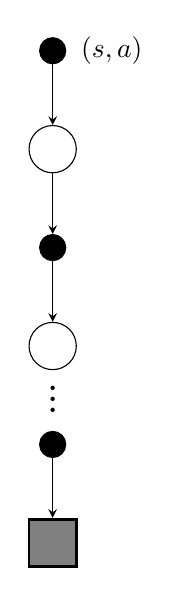
\begin{tikzpicture}[>=stealth, node distance=1.25cm]
            \tikzstyle{state} = [draw, circle, minimum size=0.6cm]
            \tikzstyle{action} = [draw, circle, minimum size=0.5mm, fill=black]
            \tikzstyle{block} = [draw, rectangle, minimum height=0.6cm, minimum width=0.6cm, fill=black!50, line width=1pt]

            \node[action] (head) {};
            \node[state, below of=head] (node1) {};
            \node[action, below of=node1] (node2) {};
            \node[state, below of=node2] (node3) {};
            \node[minimum size=0.6cm, below of=node3, yshift=0.675cm] (dots) {$\textbf{\vdots}$};
            \node[action, below of=node3] (nodeN1) {};
            \node[block, below of=nodeN1] (nodeN) {};

            \draw[->] (head.south) -- (node1.north);
            \draw[->] (node1.south) -- (node2.north);
            \draw[->] (node2.south) -- (node3.north);
            \draw[->] (nodeN1.south) -- (nodeN.north);

            \node[right of=head, xshift=-0.5cm] {$(s, a)$};
        \end{tikzpicture}
        \caption{Backup Diagram for the MC estimate of $q_{\pi}$}
        \label{fig:backup-diagram}
    \end{figure}

    \section*{Question-3}
    Solve Exercise 5.6.

    \subsection*{Solution}
    For $V(s)$, we are given
    $$V(s) = \frac{\sum_{t \in \mathcal{T}(s)} \rho_{t:T(t)-1} G_{t}}{\sum_{t \in \mathcal{T}(s)} \rho_{t:T(t)-1}}$$
    where $\mathcal{T}(s)$ is the set of all time steps at which state $s$ is visited, $T(t)$ is the time of termination
    following time step $t$, and $\rho_{t:T(t)-1}$ is the importance sampling factor of the episode following time step $t$
    till termination. \\
    $Q(s, a)$ is the value of a state-action pair, i.e. the expected return after taking action $a$ in state $s$. So,
    we define $\mathcal{T}(s, a)$ as the set of all time steps at which state-action pair $(s, a)$ is visited. Then,
    $$Q(s, a) = \frac{\sum_{t \in \mathcal{T}(s, a)} \rho_{t+1:T(t)-1} G_{t}}{\sum_{t \in \mathcal{T}(s, a)} \rho_{t+1:T(t)-1}}$$
    Note that the importance sampling factor is calculated from $t+1$ to $T(t)$, as the action at time step $t$ is $a$ (fixed).
    This can be seen as follows. Let $\rho'_{t:T(t)}$ be the importance sampling factor from $t$ to $T(t)$ for the equation of
    $Q(s, a)$. Then,
    \begin{align*}
        \rho'_{t:T(t)-1} = \frac{\prod_{k=t}^{T-1} \pi(A_{k} | S_{k})}{\prod_{k=t}^{T-1} b(A_{k} | S_{k})}
        = \prod_{k=t+1}^{T-1} \frac{\pi(A_{k} | S_{k})}{b(A_{k} | S_{k})}
        = \rho_{t+1:T(t)-1} \quad \text{(as $A_{t} = a$ is fixed)}
    \end{align*}

    \section*{Question-4}
    Solve the blackjack game problem and generate the corresponding figures.

    \subsection*{Solution}
    The solution to the blackjack game problem is given in \texttt{main.ipynb}. The figures are also generated in the notebook.

    \section*{Question-5}
    Solve Exercise 6.2.

    \subsection*{Solution}
    TD methods are often more efficient than MC methods because of a few reasons. First, TD methods are fully online
    in nature, i.e. they update the value function after every few time steps. On the other hand, MC methods update
    the value function only after the end of an episode. So, in case of very long episodes, learning is delayed.
    Second, MC methods must ignore or discount the episodes where experimental actions are taken, which slows down
    the learning. TD methods, however, learn from individual transitions and hence, are less affected by this. \\
    The scenario mentioned in the book is one where TD update is better than MC update. In it, we assume that the
    initial and terminal states have changed, but the highway states remain the same. Since the highway states remain
    the same, TD methods will accelerate the adjustment to the new state values. MC methods, on the other hand, will
    have to wait till the end of each episode to bring an average improvement to all states. This average improvement
    can also result in fluctuating value for some highway states which might not be needed.

    \section*{Question-6}
    Write the necessary code and generate the figures in Example 6.2. Answer the related questions
    asked in Exercises 6.3, 6.4, and 6.5.

    \subsection*{Solution}
    The code and figures for Example 6.2 are given in \texttt{main.ipynb}. The figures suggest that
    TD(0) methods are consistently better than MC methods. The answers to the questions are as follows.

    \subsubsection*{Exercise 6.3}
    \textbf{Why does the first episode result in change in the value of one state only?} \\[5pt]
    The first episode results in change in the value of only one state (state \texttt{A} in the book), suggesting
    that the episode ends in that state. Since $\gamma$ is 1 and intermediate rewards are zero, we can
    expect this change to be non-zero, specifically $0.5 * (-\alpha) = 0.05$, since all values were
    initialized to 0.5. \\
    If the episode ends in the right terminal state, then the value of state $\texttt{E}$ increases by
    $0.5 * \alpha = 0.05$.

    \subsubsection*{Exercise 6.4}
    \textbf{Does either algorithm perform better than the other on a specific values of $\alpha$? Do you think
    the conclusions about which one is better depends on the step-size parameter?} \\[5pt]
    No. In the plot, both algorithms are tested on very small values of the step-size parameter. A small
    value of $\alpha$ is necessary for convergence, and so, the algorithms are already tested on
    their limits. So there is no fixed value for $\alpha$ that could make a big difference for
    either method. \\
    Reducing the value of $\alpha$ after a sufficiently large number of steps might help in convergence
    of both methods.

    \subsubsection*{Exercise 6.5}
    \textbf{What is the cause of the decrease and then increase in the RMS error of TD(0) methods with different
    $\alpha$s? Is it a function of how the estimate of the value function was initialized?} \\[5pt]
    The decrease and then increase in the RMS error of TD(0) methods with different $\alpha$s is due to the
    initialization of the value function and the step-size parameter. For even smaller $\alpha$s, the
    algorithm should converge to lower and lower RMS errors. Moreover, the TD error can increase again
    when some states are overestimated and some are underestimated. This can happen when the step-size
    parameter is too large.

    \section*{Question-7}
    Write the code and generate the figures that compare the sum of rewards during episodes
    when using Q-learning and SARSA.

    \subsection*{Solution}
    The code and figures for the solution are given in \texttt{main.ipynb}.

    \section*{Question-8}
    Solve Exercise 6.12

    \subsection*{Solution}
    Even if action selection is greedy, even then Q-learning may not be equivalent to SARSA. This is because
    Q-learning works as follows:
    \begin{itemize}
        \item Take action $A_{t}$ derived from current $Q$ estimates (greedily), and observe $R_{t+1}$ and $S_{t+1}$
        \item Update $Q(S_{t}, A_{t}) = Q(S_{t}, A_{t}) + \alpha \left[ R_{t+1} + \gamma \max_{a \in \mathcal{A}(S_{t+1})} Q(S_{t+1}, a) - Q(S_{t}, A_{t}) \right]$
        \item Proceed to state $S_{t+1}'$ that maximizes the updated $Q$ estimates
    \end{itemize}
    However, SARSA works as follows:
    \begin{itemize}
        \item Take action $A_{t}$ derived from current $Q$ estimates (greedily), and observe $R_{t+1}$ and $S_{t+1}$
        \item Update $Q(S_{t}, A_{t}) = Q(S_{t}, A_{t}) + \alpha \left[ R_{t+1} + \gamma \max_{a \in \mathcal{A}(S_{t+1})} Q(S_{t+1}, a) - Q(S_{t}, A_{t}) \right]$
        \item Proceed to the already picked state, $S_{t+1}$
    \end{itemize}
    So, SARSA chooses $S_{t+1}$ with stale estimates of $Q$, while Q-learning chooses $S_{t+1}$ in
    the next iteration with the updated values of $Q$. This means that they might not necessarily pick
    the same states.

\end{document}